\section{Elliptic Curves}
\newcommand{\op}{\oplus}
\newcommand{\fanO}{\mathcal{O}}
\begin{definition}
    {Elliptic Curve} An \textit{elliptic curve} \(E\) is the set of solutions to an equation of the form \(y^2 = x^3 + ax + b\), together with a point at infinity \(\mathcal{O}\), and the condition that \(4a^{3} + 27b^{2} \ne 0\). The last condition is to prevent singular points that cross. In other words, \(4a^{3} + 27b^{2} = 0 \equiv x^{3} + ax + b\) having 3 distinct roots.
\end{definition}

\begin{center}
    \textbf{Adding Two Elliptic Curve Points} \\

    We define ``\(\oplus\)'' as mapping: \(E \times E \to E\). From this, we get \(P \oplus Q = R\).
\end{center}

Define a line through \(P \op Q\). This line will intersect the curve at a third point, \(R\). Then \(R'\) is the reflection of \(R\) over the \(y\)-axis. \(P \oplus Q = R'\).

\begin{example}
    {Adding Two Elliptic Curve Points} Given the elliptic curve \(E\colon y^{2} = x^{3} - 36x\) with \(P = (-3,9)\), \(Q = (-2,8)\). Find \(P \oplus Q\).
\end{example}

\lesol{
    \begin{enumerate}
        \item Find slope: \(m = \frac{y_{2} - y_{1}}{x_{2} - x_{1}} = \frac{8 - 9}{-2 - (-3)} = -1\).
        \item Solve the equation of line: \(y = -x + b\). Plug in \(P\): \(9 = 3 + b \implies b = 6\). Thus, \(y = -x + 6\).
        \item Plug \(y\) back into given formula:
              \begin{align*}
                  (-x + 6)^{2}                & = x^{3} - 36x \\
                  x^{2} - 12x + 36            & = x^{3} - 36x \\
                  (-x^{3}) + x^{2} + 24x + 36 & = 0           \\
                  x^{3} - x^{2} - 24x - 36    & = 0
              \end{align*}
        \item Find the roots of the equation: \(x = -3, -2, 6\). Thus, \(R = (6,0)\) and \(R' = (6,0)\). Note two important things we did here:
              \begin{itemize}
                  \item We know that two of the roots are 3 and 2 because they are given. We got the third root, \(-6\), by solving for the cubic equation.
                  \item \(R\) and \(R'\) are the same value because to find \(R'\), we reflect \(R\) over the \(y\)-axis.
              \end{itemize}
        \item Conclude: \(P \op Q = R' = (6,0)\).
    \end{enumerate}
}

\begin{theorem}
    {Addition Law Properties} Let \(E\) be an elliptic curve. Then, the addition law on \(E\) has the following properties:\[
        \begin{array}{lrclll}
            \text{(a)} & P \op \mathcal{O} & = & \mathcal{O} \op P = P    & \text{for all } P \in E.       & \text{(Identity)}    \\
            \text{(b)} & P \op (-P)        & = & (-P) \op P = \mathcal{O} & \text{for all } P \in E.       & \text{(Inverse)}     \\
            \text{(c)} & (P \op Q) \op R   & = & P \op (Q \op R)          & \text{for all } P, Q, R \in E. & \text{(Associative)} \\
            \text{(d)} & P \op Q           & = & Q \op P                  & \text{for all } P, Q \in E.    & \text{(Commutative)} \\
        \end{array}\]
    In other words, the addition law makes the points of \(E\) into an Abelian group.
\end{theorem}

\tpf{
    \begin{enumerate}
        \item \textbf{Identity:} True because \(\mathcal{O}\) lies on all vertical lines.
        \item \textbf{Inverse:} Same reason as Identity. (Also, we defined \(\mathcal{O}\) as such.)
        \item \textbf{Associative:} Ignoring because hard.
        \item \textbf{Commutative:} Line through \(P \op Q\) is the same as the line through \(Q \op P\). Hence, \(P \op Q = Q \op P\).
    \end{enumerate}
}

\subsection{Special Cases for Adding Elliptic Curve Points}

\begin{theorem}
    {Elliptic Curve Addition Algorithm} Let
    \[
        E \colon y^{2} = x^{3} + ax + b
    \]
    be an elliptic curve, and let \(P_{1}\) and \(P_{2}\) be points on \(E\).
    \begin{enumerate}[label=(\alph*)]
        \item If \(P_{1} = \mathcal{O}\), then \(P_{1} + P_{2} = P_{2}\).
        \item Otherwise, if \(P_{2} = \mathcal{O}\), then \(P_{1} + P_{2} = P_{1}\).
        \item Otherwise, write \(P_{1} = (x_{1}, y_{1})\) and \(P_{2} =(x_{2},y_{2})\).
        \item If \(x_{1} = x_{2}\) and \(y_{1} = -y_{2}\), then \(P_{1} + P_{2} = \fanO\).
        \item Otherwise, define \(\lambda\) by
              \[\lambda =
                  \begin{cases}
                      \dfrac{y_{2} - y_{1}}{x_{2} - x_{1}} & \text{if } P_{1} \ne P_{2}, \\[0.5cm]
                      \dfrac{3x_{1}^{2} + A}{2y_{1}}       & \text{if } P_{1} = P_{2},
                  \end{cases}
              \]
              and let
              \[
                  x_{3} = \lambda^{2} - x_{1} - x_{2} \qquad \text{ and } \qquad y_{3} = \lambda (x_{1} - x_{3}) - y_{1}.
              \]
              Then, \(P_{1} + P_{2} = (x_{3},y_{3})\).
    \end{enumerate}
\end{theorem}

\newcommand{\dydx}{\frac{dy}{dx}}

\begin{center}
    \textbf{Verbatim From Notes Today In Class}
\end{center}

For \(P = (x_{1}, y_{1})\), \(Q = (x_{2}, y_{2})\).
\begin{enumerate}[label=\arabic*.]
    \item \(P = Q\): This means \(x_{1} = x_{2}\), and there is no slope because \(x_{2} - x_{2} = 0\). Thus, this ``line,'' is actually a point tangent to the curve. Thus, to find the slope of the line, we need to differentiate.
    \item \(P = \mathcal{O}\) or \(Q = \mathcal{O}\): This means that the line is vertical, and the sum is the other point. In other words, \(P \op \mathcal{O} = P\).
\end{enumerate}

For the first case, consider the following example:

\begin{example}
    {Case 1} Solve for \(R'\) with the elliptic curve \(E \colon y^{2} = x^{3} - 36x\).
\end{example}

\lesol{To solve this we first need to differentiate to get the slope for our equation:
    \begin{align*}
        y^{2}   & = x^{3} - 36x                 \\
        2y\dydx & = 3x^{2} - 36                 \\
        \dydx   & = \frac{3x^{2} - 36}{2y}      \\
        \dydx   & = \frac{3(-3)^{2} - 36}{2(9)} \\
        \dydx   & = \frac{-1}{2}
    \end{align*}
    From here, we solve \(y - y_{0} = m(x - x_{0})\):
    \begin{align*}
        y - 9 & = \frac{-1}{2}(x+3)           \\
        y     & = \frac{-1}{2} + \frac{15}{2}
    \end{align*}
    Now, we can substitute our \(x\) and \(y\) values back into the original \(y^{2} = x^{3} + ax + b\):
    \begin{align*}
        \left(\frac{-1}{2}x + \frac{15}{2}\right)^{2}            & = x^{3} - 36x \\
        \frac{1}{4}x^{2} - \frac{15}{2}x + \frac{225}{4}         & = x^{3} - 36x \\
        x^{3} - \frac{1}{4}x^{2} - \frac{57}{2}x - \frac{225}{4} & = 0           \\
        (x + 3)(x+3)(x-\dfrac{25}{4})                            & = 0
    \end{align*}
    Hence, \(x = \frac{25}{4}\) and \(y = \frac{-1}{2}(\frac{25}{4}) + \frac{15}{2} - \frac{35}{8}\).

    Therefore, \(R' = P \op P = (\frac{25}{4},\frac{-35}{8})\). Note that \(\frac{35}{8}\) is negative because we flipped it along the \(y\)-axis.
}

\section{Elliptic Curves over Finite Fields}

\begin{example}
    {Elliptic Addition with Modulo} Given the elliptic curve \(E \colon y^{2} = x^{3} + 2x + 2 \pmod{17}\) with points \(P = (5,1)\) and \(Q = (16,13)\).
    \begin{enumerate}[label=(\alph*)]
        \item Find \(P \op Q\).
        \item Find \(P \op P\).
    \end{enumerate}

\end{example}

\lesol{
    \begin{enumerate}[label=(\alph*)]
        \item First, we need to find lambda. Using the formula for lambda in the \hyperref[thm:Elliptic Curve Addition Algorithm]{Elliptic Curve Addition Algorithm} part (e), first condition, we have: \(\lambda = \frac{12}{11}\), but remember, we are in modulo, so we need to find the modular inverse of 11. This is 14. Thus, \(\lambda = 12 \cdot 14 = 15\). (Note there is a quick trick of subtracting the number by 17 to get a smaller number to work with. For example, 12 and 14 are \(-5\) and \(-3\), respectively. When we multiply these, we get the same answer: 15. Hence, we can use this trick to make our calculations easier.)

              Use the formula for \(x_{3}\) and \(y_{3}\) to find the point \(R\). For \(x_{3}\):
              \begin{align*}
                  x_{3} & \equiv (15)^{2} - 5 - 16 \\
                        & \equiv (-2)^{2} - 5 - 16 \\
                        & \equiv -17               \\
                        & \equiv 0 \pmod{17}       \\
              \end{align*}
              Then, for \(y_{3}\):
              \begin{align*}
                  y_{3} & \equiv 15(5 - 0) - 1 \\
                        & \equiv (-2)(5) - 1   \\
                        & \equiv -11           \\
                        & \equiv 6 \pmod{17}
              \end{align*}
              This gives us the point \(R = (0,6)\).

        \item For \(P \op P\), we have \(P = (5,1)\). Now, we use the \hyperref[thm:Elliptic Curve Addition Algorithm]{Elliptic Curve Addition Algorithm} part (e), second condition, to find lambda. We have
              \[
                  \lambda = \frac{3(5)^{2} + 2}{2(1)} = 9 \cdot 2^{-1} \equiv 9 \cdot 9 \equiv 13 \pmod{17}.
              \]
              Now, we can find \(x_{3}\) and \(y_{3}\):
              \begin{align*}
                  x_{3} & \equiv 13^{2} - 5 - 5 \\
                        & \equiv 169 - 10       \\
                        & \equiv 159            \\
                        & \equiv 6 \pmod{17}
              \end{align*}
              For \(y_{3}\):
              \begin{align*}
                  y_{3} & \equiv 13(5 - 6) - 1 \\
                        & \equiv 13(-1) - 1    \\
                        & \equiv -14           \\
                        & \equiv 3 \pmod{17}
              \end{align*}
              This gives us the point \(R = (6,3)\).
    \end{enumerate}
}

\begin{example}
    {Set of Points \(E(\F_{p})\)} Using the same elliptic curve from the last example, \(E \colon y^{2} = x^{3} + 2x + 2 \pmod{17}\) find the set of points \(E(\F_{17})\).
\end{example}

\lesol{ For this problem, we need to find all the squares modulo 17. We can do this by squaring all the numbers from 0 to 16. \\

    \begin{minipage}{0.48\textwidth}
        \begin{enumerate}
            \item First, find all the squared values:
                  \begin{itemize}
                      \item \(0^{2} = 0\)
                      \item \(1^{2} = 1 = 16^{2}\)
                      \item \(2^{2} = 4 = 15^{2}\)
                      \item \(3^{2} = 9 = 14^{2}\)
                      \item \(4^{2} = 16 = 13^{2}\)
                      \item \(5^{2} = 8 = 12^{2}\)
                      \item \(6^{2} = 2 = 11^{2}\)
                      \item \(7^{2} = 15 = 10^{2}\)
                      \item \(8^{2} = 13 = 9^{2}\)
                  \end{itemize}
        \end{enumerate}
        Notice that the squares are symmetric about 8. This is because the curve is symmetric about the \(y\)-axis.
    \end{minipage}
    \begin{minipage}{0.48\textwidth}
        \begin{enumerate}

            \item[2.] We need to find the \(y\)-values. We need to test each of the \(x\)-values in the equation \(y^{2} = x^{3} + 2x + 2\):
                  \begin{itemize}
                      \item \(0^{3} + 2(0) + 2 = 2\)
                      \item \(1^{3} + 2(1) + 2 = 5\)
                      \item \(2^{3} + 2(4) + 2 = 12\)
                      \item \(3^{3} + 2(9) + 2 = 1\)
                      \item \(4 \to 6\)
                      \item \(5 \to 1\)
                      \item \(6 \to 9\)
                      \item \(7 \to 2\)
                      \item \(8 \to 3\)
                      \item \(9 \to 1\), \(10 \to 2\), \(11 \to 2\), \(12 \to 3\), \(13 \to 15\), \(14 \to 3\), \(15 \to 7\), \(16 \to 16\). \\
                  \end{itemize}
        \end{enumerate}
    \end{minipage}

    \begin{enumerate}
        \item[3.] Now, given a \(y\)-value, we can search for the corresponding \(x\)-value. For example, \(y = 2\) corresponds to \(x = 6\) and \(x = 11\). We find the pairs to be:

              \[
                  \begin{aligned}
                       & \mathcal{O},       \\
                       & (0, 6), (0, 11),   \\
                       & (3, 1), (3, 16),   \\
                       & (5, 1), (5, 16),   \\
                       & (6, 3), (6, 14),   \\
                       & (7, 6), (7, 11),   \\
                       & (9, 1), (9, 16),   \\
                       & (10, 6), (10, 11), \\
                       & (13, 7), (13, 10), \\
                       & (16, 4), (16, 13).
                  \end{aligned}
              \]
              This yields the set of points \(E(\F_{17})\) to be 19 points in total.
    \end{enumerate}
}

\begin{theorem}
    {Hasse} The following formula gives an estimate for the number of points on an elliptic curve over a finite field:
    \[
        p + 1 - 2\sqrt{p} \le \#E(\F_{p}) \le p + 1 + 2\sqrt{p}.
    \]
\end{theorem}

\section{The Elliptic Curve Discrete Logarithm Problem (ECDLP)}


\begin{center}
\textbf{The Double-and-Add Algorithm}
\end{center}

\begin{enumerate}
    \item Write \(n\) in binary.
    \item Repeatedly double the point \(P\) up to the highest multiple of 2 in binary representation of \(n\).
    \item Take points corresponding to binary expansion of \(n\) and add them together.
\end{enumerate}

\begin{example}
    {Double-and-Add Algorithm} Use the double-and-add algorithm to compute \(E \colon y^{2} = x^{3} + 2x + 2 \pmod{17}\) with \(p = (5,1)\) and \(n = 11\).
\end{example}

\lesol{
    \begin{enumerate}
        \item Write \(n = 11\) in binary: \(11 = 1011\).
        \item Double the point \(P\) up to the highest multiple of 2 in the binary representation of \(n\): 
        \begin{align*}
            1P &= (5,1) \\
            2P &= (6,3) \\
            4P &= (3,1) \\
            8P &= (13,7)
        \end{align*}
        \item Solve for \(11P\): 
        \begin{align*}
            11P &= 8P + 2P + P \\
            &= (13,7) + (6,3) + (5,1) \\
            &= (7,11) + (5,1) \\
            &= (13,10).
        \end{align*}
        This algorithm takes \(\leq 2n\) ``steps'' to compute \(nP\).
    \end{enumerate}
}

\begin{center}
\textbf{Ternary Expansion of \(n\)}
\end{center}

\begin{enumerate}
    \item Write \(n\) in binary.
    \item Working from smaller powers of 2 to larger powers when you have 2 or more consecutive powers or 2, we can replace: 
    \begin{align*}
        &(2^{s + 5}) + 1(2^{s + t - 1}) + 1(2^{s + t - 2}) + \cdots + 1(2^{s}) \\
        &= 2^{s + t} - 2^{s}.
    \end{align*}
    This allows us to ``cancel out'' middle terms of consecutive powers of 2. We take the next largest power of 2, for a string of 2s, and subtract the next smallest power of 2.
\end{enumerate}

\begin{example}
    {Ternary Expansion} Find the ternary expansion of 11.
\end{example}

\lesol{
    \begin{enumerate}
        \item Write 11 in binary: 11 = 1011.
        \item Replace the binary expansion with the ternary expansion: 
        \begin{align*}
            11 &= 8 + 2 + 1 \\
            &= 1(8) + 1(4)  + {1(2)} + 1(1) \\
            &= 8 + 4 + \slashed{1(2)} - 1 \\
            &= 11.
        \end{align*}
    \end{enumerate}
}

\section{Elliptic Curve Cryptography}

\subsection{Elliptic Curve Diffie-Hellman Key Exchange}

\begin{table}[h!]
    \centering
    \begin{tabular}{@{}p{0.9\textwidth}l@{}}
        \toprule
        \multicolumn{2}{c}{\parbox[t]{0.9\textwidth}{\centering \textbf{Public parameter creation}}} \\ \midrule
        \multicolumn{2}{c}{\parbox[t]{0.9\textwidth}{\centering A trusted party chooses and publishes a large prime \(p\), an elliptic curve \(E\) over \(\F_{p}\) and a point \(P\) in \(E(\F_{p})\). }}        \\ \toprule
        \multicolumn{2}{c}{\parbox[t]{0.9\textwidth}{\centering \textbf{Private Computations}}} \\ \midrule
        \multicolumn{1}{c}{\parbox[t]{0.45\textwidth}{\centering \textbf{Alice}}} & \multicolumn{1}{c}{\parbox[t]{0.45\textwidth}{\centering \textbf{Bob}}} \\ \midrule
        \multicolumn{1}{l}{\parbox[t]{0.45\textwidth}{\raggedright Chooses a secret integer \(n_{A}\). \\ Computes the point \(Q_{A} = n_{A}P\)}} & \multicolumn{1}{c}{\parbox[t]{0.45\textwidth}{\raggedright Chooses a secret integer \(n_{B}\). \\ Computes the point \(Q_{B} = n_{B}P\) }} \\ \midrule
        \multicolumn{2}{c}{\parbox[t]{0.9\textwidth}\centering\textbf{Public Exchange of Values}} \\ \midrule
        \multicolumn{1}{l}{\parbox[t]{0.45\textwidth}{\raggedright Alice sends \(Q_{A}\) to Bob}} &  \\ \midrule
        \multicolumn{1}{l}{\parbox[t]{0.45\textwidth}}                               & \multicolumn{1}{r}{\parbox[t]{0.45\textwidth}{\raggedright Bob sends \(Q_{B}\) to Alice}} \\ \toprule
        \multicolumn{2}{c}{\parbox[t]{0.9\textwidth}{\centering\textbf{Further Private Computations}}} \\ \midrule
        \multicolumn{1}{l}{\parbox[t]{0.45\textwidth}{\raggedright Computes the point \(n_{A}Q_{B}\). }} & \multicolumn{1}{c}{\parbox[t]{0.45\textwidth}{\raggedright  Computes the point \(n_{B}Q_{A}\). }} \\\midrule 
        \multicolumn{2}{c}{\parbox[t]{0.9\textwidth}\centering Their shared secret value is \(n_{A}Q_{B} = n_{A}(n_{B}P) = n_{B}(n_{A}P) = n_{B}Q_{A}\).} 
        \\ \bottomrule
    \end{tabular}
    \caption{Diffie-Hellman Key Exchange Using Elliptic Curves} 
\end{table}

\begin{example}
    {Elliptic Curve Diffie-Hellman Key Exchange} Given the elliptic curve \(E \colon y^{2} \equiv x^{3} + x + 6 \pmod{11}\) with point \(p = (5,9)\), Alice's private key \(n_{A} = 4\), and Bob's private key \(n_{B} = 7\), find the shared secret key. Use this website: \href{https://andrea.corbellini.name/ecc/interactive/modk-add.html}{Elliptic Curve Calculator}.
\end{example}

\lesol{ 
    First, we need to find \(Q_{A}\) and \(Q_{B}\). For \(Q_{A}\), we have \(n_{A} = 4\), so we need to find \(4P\). Using the double-and-add algorithm, we have \(n = 4 = 100\). Now, we need to solve for \(2P\) and \(4P\):
    \begin{align*}
        \lambda &= \frac{3(5)^{2} + 1}{2(9)} = \frac{76}{18} = 10 \cdot 18^{-1} \equiv -1 \cdot 7 \equiv -7 \equiv 4 \pmod{11} \\
    \end{align*}
    Now we can find \(x_{3}\) and \(y_{3}\). First, \(x_{3}\):
    \begin{align*}
        x_{3} &\equiv 4^{2} - 5 - 5 \\
        &\equiv 16 - 10 \\
        &\equiv 6 \pmod{11}.
    \end{align*}
    For \(y_{3}\):
    \begin{align*}
        y_{3} &\equiv 4(5 - 6) - 9 \\
        &\equiv 4(-1) - 9 \\
        &\equiv -4 - 9 \\
        &\equiv 9 \pmod{11}.
    \end{align*}
    Thus, \(2P = (6,9)\). Using the same process, we find that \(Q_{A} = 2(2P) = 2(6,9) = (3,6)\). 
    \begin{align*}
        1P &= (5,9) \\
        2P &= (6,9) \\
        4P &= (3,6).
    \end{align*} 

    Similarly, for \(7Q_{B} \Rightarrow 7P = (2,4)\). 
    
    From the image below, we can see that when we take the point \(n_{A}Q_{B} \Rightarrow 4 \cdot (2,4)\), we get the point \((10,9)\). Then, when we take the point \(n_{B}Q_{A} \Rightarrow 7 \cdot (3,6)\), we get the point \((10,9)\). Thus, the shared secret key is \((10,9)\).


\begin{center}
        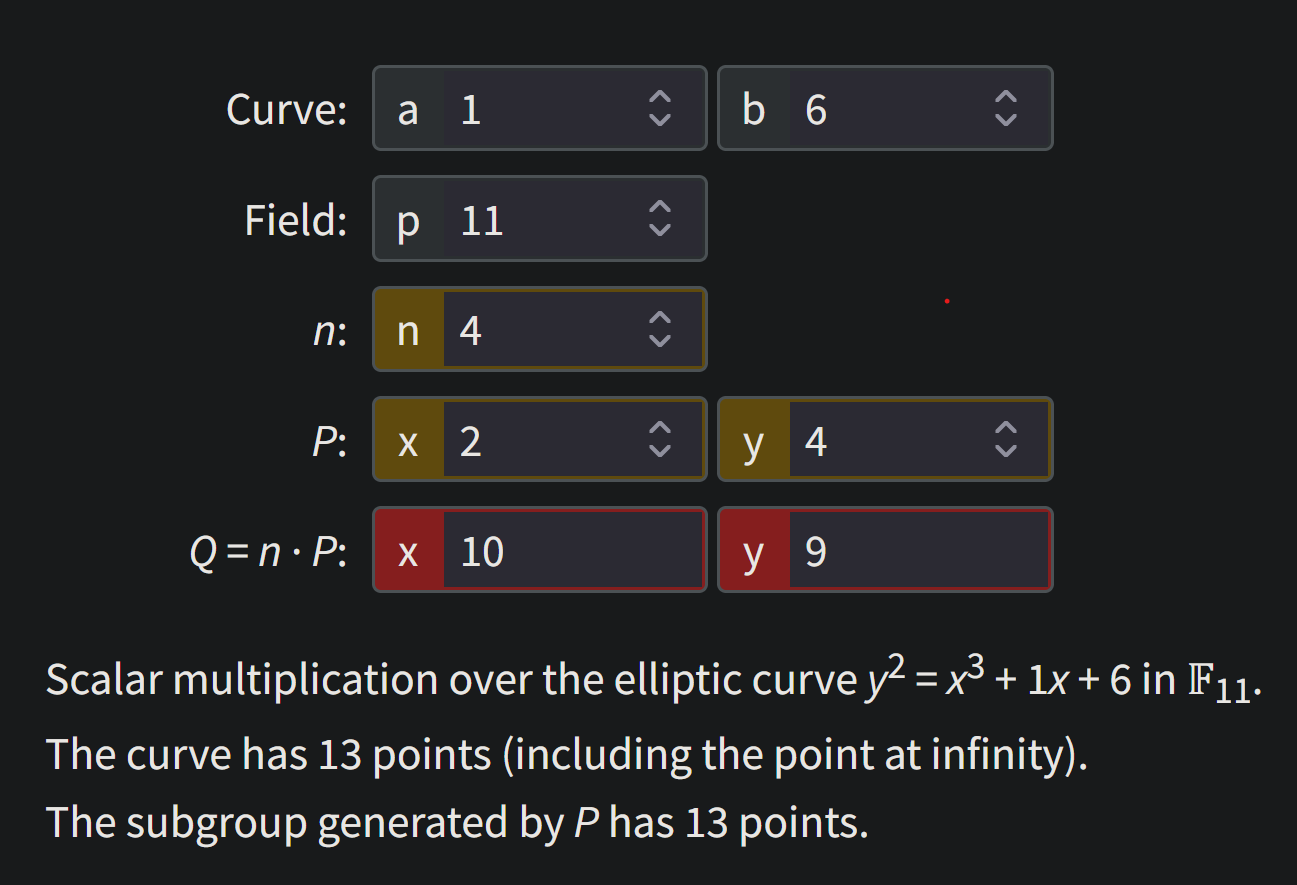
\includegraphics[width=0.4\textwidth]{images/finding_shared_key.png} \hfill
        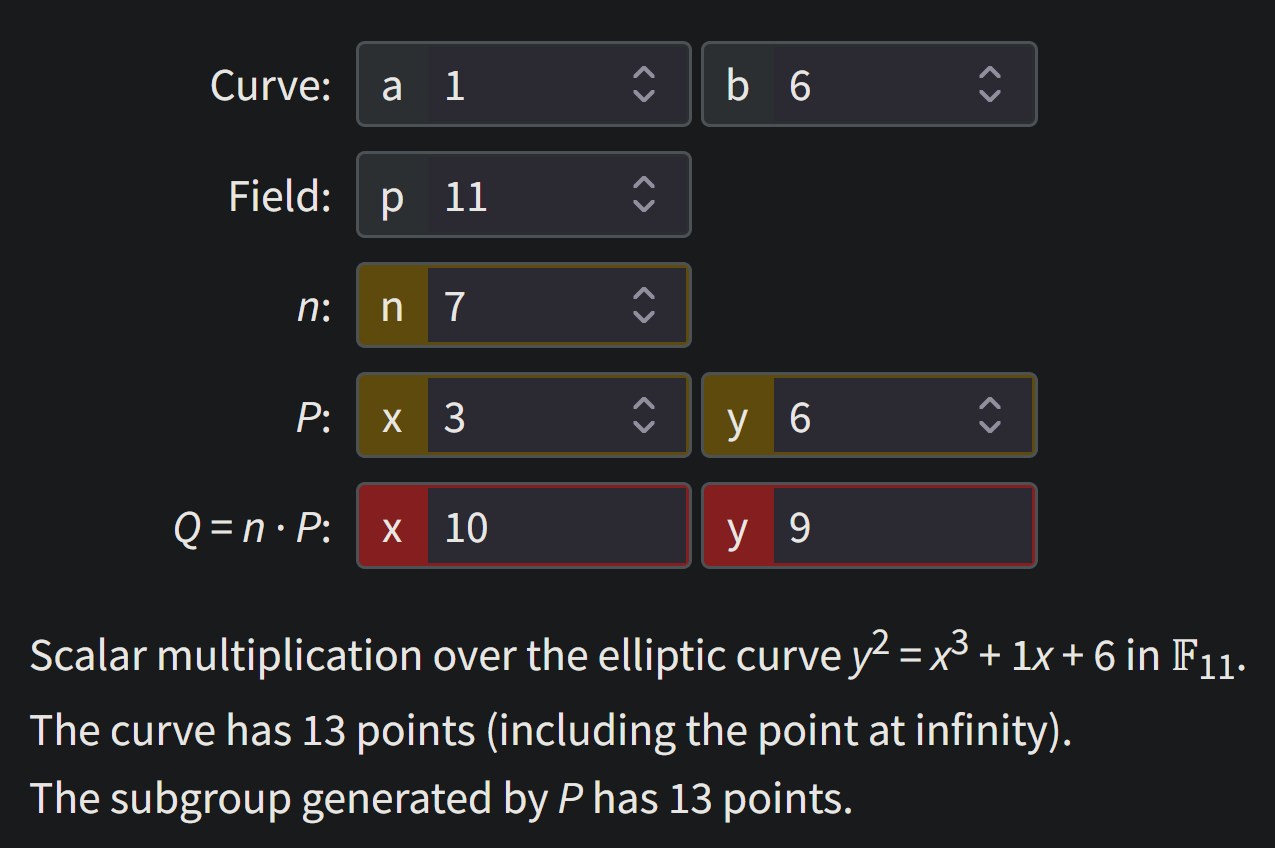
\includegraphics[width=0.4\textwidth]{images/finding_shared_key_2.png} \\
\end{center}
}

% \begin{example}
%     {Only Using the \(x\)-Coordinate} (Use the previous problem's values) Alice and Bob decide they only want to use the \(x\)-coordinate of their public key to preserve the amount of information they share. Show that they will get the same shared secret key.
% \end{example}

% \lesol{
%     We have \(Q_{A} = 3\) and \(Q_{B} = 2\). To get \(y_{1}\) from 
%     \[
%     y_{B}^{2} = x_{B}^{3} + x_{B} + 6 = 2^{3} + 2 + 6 = 16 + 2 + 6 = 24 \equiv 2 \pmod{11},
%     \]
%     we need to calculate the square root of 2 modulo 11. We get:
%     \[
%     y_{B}  = 2^{11 + 1} / 4
%     \]
% }
\newpage
\subsection{Elgamal Encryption Using Elliptic Curves}

\begin{table}[h]
    \centering
    \begin{tabular}{@{}p{0.9\textwidth}l@{}}
        \toprule
        \multicolumn{2}{c}{\parbox[t]{0.9\textwidth}{\centering \textbf{Public parameter creation}}}                                                                                  \\ \midrule
        \multicolumn{2}{c}{\parbox[t]{0.9\textwidth}{\centering A trusted party chooses and publishes a large prime \(p\), an elliptic curve \(E\) over \(\F_{p}\), and a point \(P\) in \(E(\F_{p})\).}} \\ \midrule
        \multicolumn{2}{c}{\parbox[t]{0.9\textwidth}{\centering \textbf{Key creation}}}                                                                                               \\ \midrule
        \multicolumn{1}{c}{\parbox[t]{0.45\textwidth}{\centering \textbf{Alice}}} & \multicolumn{1}{c}{\parbox[t]{0.45\textwidth}{\centering \textbf{Bob}}}                           \\ \midrule
        \multicolumn{1}{l}{\parbox[t]{0.45\textwidth}{Choose private key \(n_{A}\). \\ Compute \(Q_{A} = n_{A}P\) in \(E(\F_{p})\). \\ Publish the public key \(Q_{A}\).}} &  \\ \midrule
        \multicolumn{2}{c}{\parbox[t]{0.9\textwidth}\centering\textbf{Encryption}}                                                                                                    \\ \midrule
        \multicolumn{1}{l}{\parbox[t]{0.45\textwidth}}                            & \multicolumn{1}{r}{\parbox[t]{0.45\textwidth}{\raggedright Choose plaintext \(M \in E(\F_{p})\).                \\ Choose random element \(k\). \\ Use Alice's public key \(Q_{A}\) to \\ \quad compute \(C_1 = kP \in E(\F_{P})\) \\ \quad and \(C_2 = M + kQ_{A} \in E(\F_{P})\). \\ Send ciphertext \((C_1,C_2)\) to Alice.}}                                            \\ \midrule
        \multicolumn{2}{c}{\parbox[t]{0.9\textwidth}{\centering\textbf{Decryption}}}                                                                                                  \\ \midrule
        \multicolumn{1}{l}{\parbox[t]{0.45\textwidth}{Compute \(C_{2} - n_{A}C_{1} \in E(\F_{P})\). \\  This quantity is equal to \(M\).}}                     &                                                                                             \\ \bottomrule
    \end{tabular}
    \caption{Elgamal Key Creation, Encryption, and Decryption with Elliptic Curves}
\end{table}

\begin{example}
    {Elgamal Encryption Using Elliptic Curves} Given the elliptic curve \(E \colon y_{2} \equiv x_{3} + 7x + 4 \pmod{17}\) with \(P = (3,1)\), \(n_{A} = 15\), \(M = (16,8)\), and \((K = 5)\), find \(Q_{A}\), and encrypt and decrypt the message.
\end{example}

\lesol{
    We find \(Q_{A}\) to be \((11,16)\)
    \[
    C_{1} = 5(3,1) = (0,15).
    \]
    Then, 
    \[
    C_{2} = (16,8) + 5(11,16) = (3,1).
    \]
    Alice can decrypt the message by computing:
    \[
    (3,1) \ominus 15(0,15) = (3,1) \ominus (2,14) = (3,1) \oplus (2,3) = (16,8).
    \]
    (Note the subtraction is just taking \(-y\).)
}